\documentclass{beamer}

%encoding
%--------------------------------------
\usepackage[T1]{fontenc}
\usepackage[utf8]{inputenc}
%--------------------------------------

%Portuguese-specific commands
%--------------------------------------
\usepackage[portuguese]{babel}
%--------------------------------------

\usepackage{amsmath}

\usepackage{tikz}
\usepackage{pgfplots}
\pgfplotsset{compat = newest}
\usepgfplotslibrary{colormaps}

%Hyphenation rules
%--------------------------------------
\usepackage{hyphenat}
\hyphenation{mate-mática recu-perar}
%--------------------------------------

\usepackage{wrapfig}
\usepackage{graphicx}
\usepackage{biblatex}
\usepackage{hyperref}
\hypersetup{
    colorlinks=true,
    linkcolor=blue,
    filecolor=magenta,      
    urlcolor=cyan,
}
\urlstyle{same}

\usepackage[document]{ragged2e}

\usepackage[font=scriptsize,labelformat=empty,labelfont=it,textfont=it]{caption}
 \def\vec{\mathaccent "017E\relax }

\addbibresource{latex-beamer-template.bib}

\graphicspath{ {images/} {.images} }

\usetheme{Warsaw}
\usecolortheme{seagull}

\setbeamertemplate{headline}{}
\setbeamertemplate{section in toc}[sections numbered]
\setbeamertemplate{subsection in toc}[subsections numbered]

\setbeamercolor{block body}{bg=yellow!30}
\setbeamercolor{block title}{bg=yellow!40}

\setbeamercolor{block body alerted}{bg=red!10}
\setbeamercolor{block title alerted}{bg=red!20}

\setbeamercolor{block body example}{bg=green!10}
\setbeamercolor{block title example}{bg=green!20}

% Information to be included in the title page:
\title{A Independência do Caminho na Integral do Trabalho}
\subtitle{Trabalho 1 - Grupo 16}

\author [Alex, Caio, Pedro]{
    \small Alex Campbell e Souza - Engenharia de Sistemas \\ 
    Caio Lucas Gomes Silva - Matemática \\ 
    Pedro Mansur Gamarano - Matemática
}

\institute[]{
    \large UFMG \\
    \footnotesize Universidade Federal de Minas Gerais \\
    \small Fundamentos de Eletromagnetismo
}


\date{\today}

\begin{document}

\frame{\titlepage}

\frame{\tableofcontents}

\section{Introdução}
\begin{frame}
    \frametitle{O Trabalho (W)}
    
    O trabalho é a grandeza física associada a mudança de energia. 
    Ele acontece quando aplicamos uma força sobre um corpo e este sofre um deslocamento. 
    O trabalho de uma força constante pode ser escrito como: 
    \begin{equation}\label{eq:trabalho-constante}
    W = F * d * cos(\theta)
    \end{equation}

    Já o trabalho de uma força não constante pode ser escrito como: 
    \begin{equation}\label{trabalho-nao-constante}
    W = \mathit{\int_{a}^b \vec{F} d\vec{r}}
    \end{equation}

\end{frame}

\begin{frame}
    \frametitle{Campos Elétricos e Campos Conservativos}
    
    O \textbf{método da idependência do caminho} é possivel apenas em campos conservativos. 
    Um campo é conservativo quando ele é obtido atraves do cálculo do vetor gradiente de uma função. 
    O campo elétrico é um exemplo de campo conservativo.

\end{frame}

\begin{frame}
    \frametitle{Campos Elétricos e Campos Conservativos}
    
    
    \begin{wrapfigure}{r}{0.4\textwidth} %this figure will be at the right
        \vspace{-35pt}
        \centering
        \caption{}
        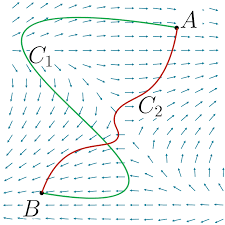
\includegraphics[width=0.30\textwidth]{grafico-trabalho.png}
        \label{fig:grafico-trabalho}
    \end{wrapfigure}
    
    A \textbf{independencia do caminho} diz que, em campos conservativos, quaisquer integrais de 
    linha que possuem os mesmos pontos inicial e final resultam em um mesmo valor, independente da curva entre eles. 
    Utilizando o trabalho como exemplo:  
    \hfill \break
    \hfill \break
    %\begin{equation}\label{trabalho-nao-constante}
    $    
        W = \mathit{\int_{c_1} \vec{F} d\vec{r}} = f(b) - f(a) 
        \hfill \break
        W = \mathit{\int_{c_2} \vec{F} d\vec{r}} = f(b) - f(a) 
    $
    %\end{equation}

\end{frame}

\section{Exemplo}

\begin{frame}
    \frametitle{Exemplo} 

    \begin{wrapfigure}{r}{0.3\textwidth} %this figure will be at the right
        \vspace{-35pt}
        \centering
        \caption{}
        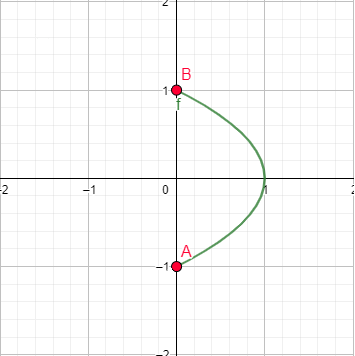
\includegraphics[width=0.30\textwidth]{grafico-exemplo-1.png}
        \label{fig:grafico-exemplo1}
    \end{wrapfigure}

    Dado o campo conservativo $ F(x, y) = ( x^2, \cos(y) ) $, calcule o trabalho de deslocamento sobre a 
    curva $ c_1(t) = ( 1 - t^2, t ) $ que tem ponto inicial $ A(0, -1) $ e final $ B(0, 1) $:
    \hfill \break
    \hfill \break
    $
        \int{} \vec{F} d\vec{r} =  
        \begin{cases}
            F(x, y) = ( x^2, \cos(y) ),\\
            c_1 = ( 1 - t^2, t) &sendo \; t \; \epsilon \; [ -1, 1 ] \; e\\
            c_1 = ( 0, t)       &sendo \; t \; \epsilon \; [ -1, 1 ] \\
        \end{cases}
    $

\end{frame}

\begin{frame}
    \frametitle{Resolução - Exemplo} 
    Usando $ c_1 $: \\
    
    $ F(x, y) = ( x^2, \cos(y) ) = (( 1 - t^2 ), \cos(t) ) $
    \hfill \break
    $ d\vec{r} $
    \hfill \break
    $ c(t) = ( 1 - t^2, t ) = ( 1 - (-1)^2 , 1) = ( 0, 1 ) $
    \hfill \break

    \begin{align*}   
    \int_{c_1} \vec{F} d\vec{r} &= \int_{-1}^1 (( 1 - t^2)^2, \cos(t) ) \cdot ( 0, 1 ) dt \\
    \int_{c_1} \vec{F} d\vec{r} &= \int_{-1}^1 \cos(t) dt  \\
    \int_{c_1} \vec{F} d\vec{r} &= \sin(t)\vert_{-1}^{1} \\
    \int_{c_1} \vec{F} d\vec{r} &= \sin(1) - \sin(-1) \\
    \int_{c_1} \vec{F} d\vec{r} &= 2 * \sin(1) \\
    \end{align*}

\end{frame}

\begin{frame}
    \frametitle{Exemplo} 

    \begin{wrapfigure}{r}{0.3\textwidth} %this figure will be at the right
        \vspace{-35pt}
        \centering
        \caption{}
        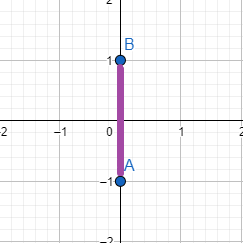
\includegraphics[width=0.30\textwidth]{grafico-exemplo-2.png}
        \label{fig:grafico-exemplo1}
    \end{wrapfigure}

    Utilizando a independencia do caminho podemos calcular a mesma integral utilizando 
    a reta $ c_2(t) = ( 0, t) $, que liga os pontos $ A $ e $ B $.

\end{frame}

\begin{frame}
    \frametitle{Resolução - Exemplo} 
    Usando $ c_2 $: \\
    
    $ F(x, y) = ( x^2, \cos(y) ) = ( 0, \cos(t) ) $
    \hfill \break
    $ d\vec{r} $
    \hfill \break
    $ c(t) = ( 0, t ) = ( 0, 1 ) $
    \hfill \break
    
    \begin{align*}   
    \int_{c_2} \vec{F} d\vec{r} &= \int_{-1}^1 (0, \cos(t) ) \cdot ( 0, 1 ) dt \\
    \int_{c_2} \vec{F} d\vec{r} &= \int_{-1}^1 \cos(t) dt  \\
    \int_{c_2} \vec{F} d\vec{r} &= \sin(t)\vert_{-1}^{1} \\
    \int_{c_2} \vec{F} d\vec{r} &= \sin(1) - \sin(-1) \\
    \int_{c_2} \vec{F} d\vec{r} &= 2 * \sin(1) \\
    \end{align*}
    
\end{frame}

\begin{frame}
    \frametitle{Conclusão} 
    Esta técnica pode ser muito útil para resolver problemas complexos envolvendo forças conservativas. 
    Uma ferramenta importante dentro do estudo do eletromagnetismo.
    \hfill \break
    \hfill \break
    O código fonte deste documento pode ser encontrado em:
    \hfill \break
    \url{https://tinyurl.com/yya8nuau}

\end{frame}

%\nocite{*}
\begin{frame}[noframenumbering,plain,allowframebreaks]{Referências}
    \begin{thebibliography}{10}
        \bibitem{young}[Física III - Eletromagnetismo, 2015]
        YOUNG - FREEDMAN.
        \newblock 9788543018157,
        \newblock Pearson.
        
        \bibitem{khanacademy}[Campos vetoriais conservativos]
        \newblock \url{https://pt.khanacademy.org/math/multivariable-calculus/integrating-multivariable-functions/line-integrals-in-vector-fields-articles/a/conservative-fields}
             
        \bibitem{youtube1}[Integrais de Linha - Independência do Caminho]
        \newblock Responde Aí.
        \newblock \url{https://www.youtube.com/watch?v=ONpa0kJ5TAs}
             
        \bibitem{youtube2}[Integral de Linha de Função Vetorial (VETORIAL)]
        \newblock Toda a Matemática
        \newblock \url{https://www.youtube.com/watch?v=r_NwdXff0Ok}

        \bibitem{youtube2}[Campo Conservativo (VETORIAL)]
        \newblock Toda a Matemática
        \newblock \url{https://www.youtube.com/watch?v=R1xmPwTq7Q0}
        
    \end{thebibliography}
\end{frame}


\end{document}